%!TEX root = handout.tex

\newpage
\section{OpenSWATH}
\subsection{Introduction}

OpenSWATH~\cite{Rost2014fd} allows the analysis of LC-MS/MS DIA (data independent acquisition) data using the approach described by Gillet \textit{et~al.}~\cite{Gillet2012Targeted}. The DIA approach described there uses 32 cycles to iterate through precursor ion windows from 400-426 Da to 1175-1201 Da and at each step acquires a complete, multiplexed fragment ion spectrum of all precursors present in that window. After 32 fragmentations (or 3.2 seconds), the cycle is restarted and the first window (400-426 Da) is fragmented again, thus delivering complete ``snapshots'' of all fragments of a specific window every 3.2 seconds. \\

\noindent The analysis approach described by Gillet et al. extracts ion traces of specific fragment ions from all MS2 spectra that have the same precursor isolation window, thus generating data that is very similar to SRM traces.

\subsection{Installation of OpenSWATH}
OpenSWATH has been fully integrated since OpenMS 1.10 \cite{Kohlbacher2007,Sturm2008,Bertsch2011OpenMS,Rost2016,Pfeuffer2017}).

\subsection{Installation of mProphet}
mProphet (\url{http://www.mprophet.org/}) \cite{Reiter2011MProphet} is available as standalone script in \directory{External\_Tools/mProphet/}. 
R (\url{http://www.r-project.org/}) and the package MASS (\url{http://cran.r-project.org/web/packages/MASS/}) are further required to execute mProphet. 
Please obtain a version for either Windows, Mac or Linux directly from CRAN. \\

\noindent PyProphet, a much faster reimplementation of the mProphet algorithm is available from PyPI (\url{https://pypi.python.org/pypi/pyprophet/}). The usage of pyprophet instead of mProphet is suggested for large-scale applications. \\ %For furhter installtion instruction please have a look below. 
\newline \noindent mProphet will be used in this tutorial.

\subsection{Generating the Assay Library}
\subsubsection{Generating TraML from transition lists}
OpenSWATH requires an assay library to be supplied in the TraML format \cite{Deutsch2012TraMLA}. To enable manual editing of transition lists, the TOPP tool \OPENMSTOOL{TargetedFileConverter} is available, which uses tab separated files as input. Example datasets are provided in \directory{Example\_Data/OpenSWATH/assay/}. Please note that the transition lists need to be named \texttt{.tsv}.

\noindent The header of the transition list contains the following variables (with example values in brackets):

\begin{description}
  \item[Required Columns:]
  \item[\texttt{PrecursorMz}] \hfill \\
  The mass-to-charge (m/z) of the precursor ion. (924.539)
  \item[\texttt{ProductMz}] \hfill \\
  The mass-to-charge (m/z) of the product or fragment ion. (728.99)
   \item[\texttt{LibraryIntensity}] \hfill \\
  The relative intensity of the transition. (0.74)
  \item[\texttt{NormalizedRetentionTime}] \hfill \\
  The \textbf{normalized} retention time (or iRT) \cite{Escher2012Using} of the peptide. (26.5)
  \newline
  \item[Targeted Proteomics Columns:]
  \item[\texttt{ProteinId}] \hfill \\
  A unique identifier for the protein. (AQUA4SWATH\_HMLangeA)
  \item[\texttt{PeptideSequence}] \hfill \\
  The unmodified peptide sequence. (ADSTGTLVITDPTR)
  \item[\texttt{ModifiedPeptideSequence}] \hfill \\
  The peptide sequence with UniMod modifications. (ADSTGTLVITDPTR(UniMod:267))
  \item[\texttt{PrecursorCharge}] \hfill \\
  The precursor ion charge. (2)
  \item[\texttt{ProductCharge}] \hfill \\
  The product ion charge. (2)
  \newline
  \item[Grouping Columns:]
  \item[\texttt{TransitionGroupId}] \hfill \\
  A \textbf{unique} identifier for the transition group.\\
  (AQUA4SWATH\_HMLangeA\_ADSTGTLVITDPTR(UniMod:267)/2)
  \item[\texttt{TransitionId}] \hfill \\
  A \textbf{unique} identifier for the transition.\\
  (AQUA4SWATH\_HMLangeA\_ADSTGTLVITDPTR(UniMod:267)/2\_y8)
  \item[\texttt{Decoy}] \hfill \\
  A binary value whether the transition is target or decoy. (target: 0, decoy: 1)
  \item[\texttt{PeptideGroupLabel}] \hfill \\
  Which label group the peptide belongs to. \\
  \item[\texttt{DetectingTransition}] \hfill \\
  Use transition for peak group detection. (1)\\
  \item[\texttt{IdentifyingTransition}] \hfill \\
  Use transition for peptidoform inference using IPF. (0)\\
  \item[\texttt{QuantifyingTransition}] \hfill \\
  Use transition to quantify peak group. (1)\\
\end{description}

\noindent For further instructions about generic transition list and assay library generation please see \url{http://openswath.org/en/latest/docs/generic.html}. \\

\noindent To convert transitions lists to TraML, use the \OPENMSTOOL{TargetedFileConverter}: Please use the absolute path to your OpenMS installation. \\

\begin{description}
  \item[Linux or Mac] \hfill \\
    On the Terminal:
    \begin{lstlisting}
TargetedFileConverter -in OpenSWATH_SGS_AssayLibrary_woDecoy.tsv -out OpenSWATH_SGS_AssayLibrary_woDecoy.TraML
  \end{lstlisting}
  \item[Windows] \hfill \\
    On the TOPP command line:
    \begin{lstlisting}
TargetedFileConverter.exe -in OpenSWATH_SGS_AssayLibrary_woDecoy.tsv -out OpenSWATH_SGS_AssayLibrary_woDecoy.TraML
  \end{lstlisting}
\end{description}

\subsubsection{Appending decoys to a TraML file}
In addition to the target assays, OpenSWATH requires decoy assays in the library which are later used for classification and error rate estimation. For the decoy generation it is crucial that the decoys represent the targets in a realistic but unnatural manner without interfering with the targets. The methods for decoy generation implemented in OpenSWATH include 'shuffle', 'pseudo-reverse', 'reverse' and 'shift'. To append decoys to a TraML, the TOPP tool \OPENMSTOOL{OpenSwathDecoyGenerator} can be used: Please use the absolute path to your OpenMS installation.

\begin{description}
  \item[Linux or Mac] \hfill \\
    On the Terminal:
    \begin{lstlisting}
OpenSwathDecoyGenerator -in OpenSWATH_SGS_AssayLibrary_woDecoy.TraML -out OpenSWATH_SGS_AssayLibrary.TraML -method shuffle -switchKR false
  \end{lstlisting}
  \item[Windows] \hfill \\
    On the TOPP command line:
    \begin{lstlisting}
  OpenSwathDecoyGenerator.exe -in OpenSWATH_SGS_AssayLibrary_woDecoy.TraML -out OpenSWATH_SGS_AssayLibrary.TraML -method shuffle -switchKR false
  \end{lstlisting}
\end{description}

\subsection{OpenSWATH KNIME}
An example KNIME workflow for OpenSWATH is supplied in \directory{Workflows/} (Fig.~\ref{fig:openswath}). The example dataset can be used for this workflow (filenames in brackets):

\begin{enumerate}
  \item Open \directory{Workflows /OpenSWATH.knwf} in KNIME: \menu{File > Import KNIME Workflow...}.
  \item Select the normalized retention time (iRT) assay library in TraML format by double-clicking on node \menu{Input File > iRT Assay Library}.\\
  (\directory{Example\_Data/OpenSWATH/assay/OpenSWATH\_iRT\_AssayLibrary.TraML})
  \item Select the SWATH MS data in mzML format as input by double-clicking on node \menu{Input File > SWATH-MS files}.\\
  (\directory{Example\_Data/OpenSWATH/data/split\_napedro\_L120420\_010\_SW-*.nf.pp.mzML})
  \item Select the target peptide assay library in TraML format  as input by double-clicking on node \menu{Input Files > Assay Library}.\\
  (\directory{Example\_Data/OpenSWATH/assay/OpenSWATH\_SGS\_AssayLibrary.TraML})
  \item Set the output destination by double-clicking on node \menu{Output File}.\\
  \item Run the workflow.
\end{enumerate}

\noindent The resulting output can be found at your selected path, which will be used as input for mProphet. Execute the script on the Terminal (Linux or Mac) or cmd.exe (Windows) in \directory{Example\_Data/OpenSWATH/result}. Please use the absolute path to your R installation and the result file:

\begin{lstlisting}
R --slave --args bin_dir=../../../External_Tools/mProphet/ mquest=OpenSWATH_quant.tsv workflow=LABEL_FREE num_xval=5 run_log=FALSE write_classifier=1 write_all_pg=1 < ../../../External_Tools/mProphet/mProphet.R
\end{lstlisting}
or for windows
\begin{lstlisting}
"C:\Program Files\R\R-3.5.1\bin\x86\R.exe" --slave --args bin_dir=../../../External_Tools/mProphet/ mquest=OpenSWATH_quant.tsv workflow=LABEL_FREE num_xval=5 run_log=FALSE write_classifier=1 write_all_pg=1 < ../../../External_Tools/mProphet/mProphet.R
\end{lstlisting}

% begin comment pyopenms
\begin{comment}
\noindent If you have a valid python installation, pyProphet can be used. Further instructions the installation of python can be found in the pyOpenMS section. 

\noindent Installation of the current stable version:
\begin{lstlisting}
pip install pyprophet
\end{lstlisting}

\noindent The following command should provide similar results to the mProphet script:
\begin{lstlisting}
pyprophet score --in OpenSWATH_quant.tsv --out OpenSWATH_quant_scoring.tsv --group_id transition_group_id --pi0_lambda 1e-6 1e-2 1e-6
\end{lstlisting}
\end{comment}
% end comment pyopenms

\noindent The main output will be called\\
\directory{OpenSWATH/result/mProphet\_all\_peakgroups.xls}\\
with statistical information available in\\
\directory{OpenSWATH/result/mProphet.pdf}.\\

\noindent Please note that due to the semi-supervised machine learning approach of mProphet the results differ slightly when mProphet is executed several times. \\

\begin{figure}[!ht]
  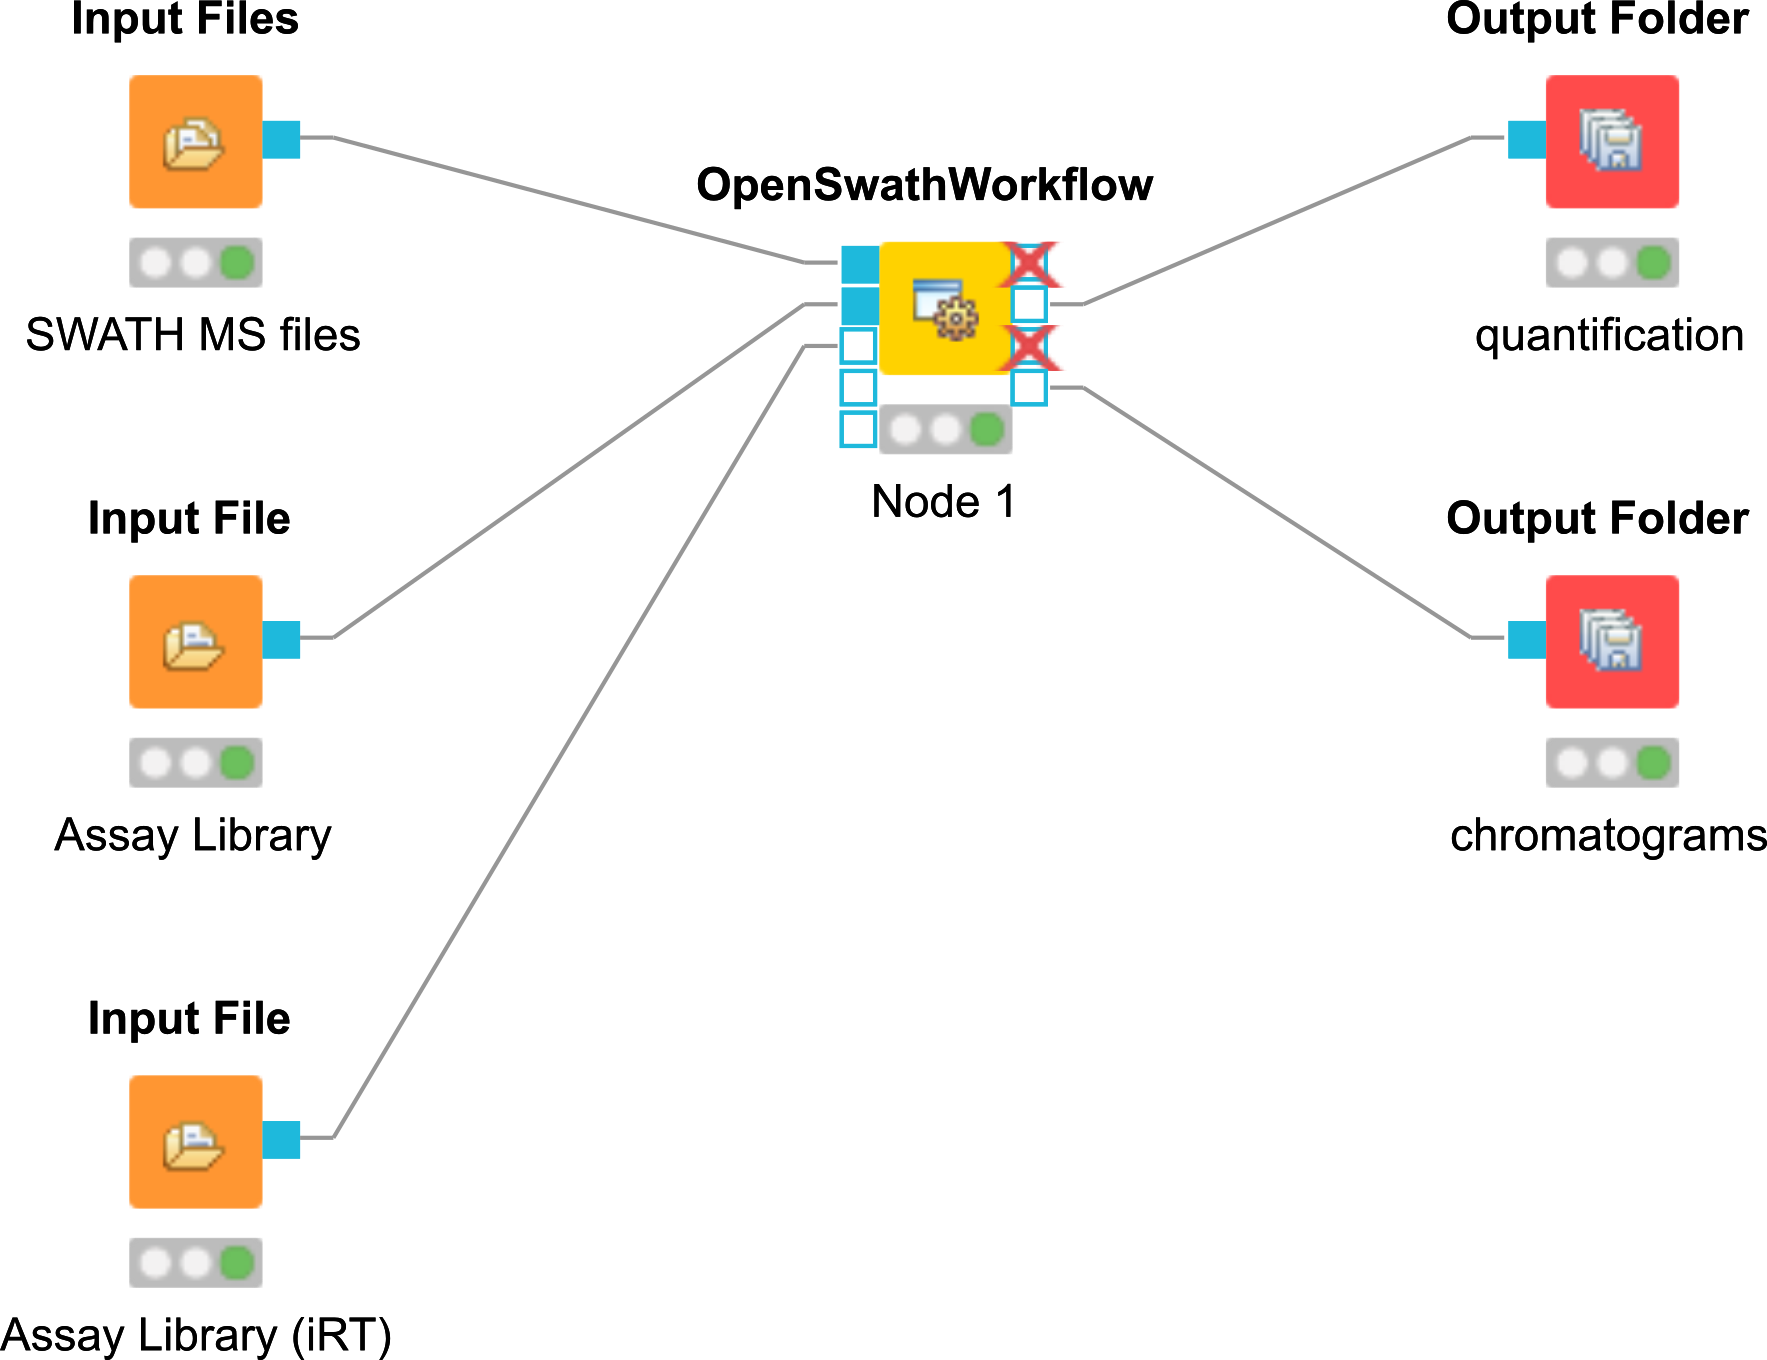
\includegraphics[width=0.7\textwidth]{graphics/openswath/OpenSWATHWF.png}
  \caption{OpenSWATH KNIME Workflow.}
  \label{fig:openswath}
\end{figure}

\noindent Additionally the chromatrogam output (.mzML) can be visualized for inspection with \OPENMSTOOL{TOPPView}. \\

\noindent For additional instructions on how to use pyProphet instead of mProphet please have a look at the PyProphet Legacy Workflow \url{http://openswath.org/en/latest/docs/pyprophet_legacy.html}. If you want to use the SQLite-based workflow in your lab in the future, please have a look here: \url{http://openswath.org/en/latest/docs/pyprophet.html}. The SQLite-based workflow will not be part of the tutorial. \\

\subsection{From the example dataset to real-life applications}
The sample dataset used in this tutorial is part of the larger SWATH MS Gold Standard (SGS) dataset which is described in the publication of Roest et al.~\cite{Rost2014fd}.
It contains one of 90 SWATH-MS runs with significant data reduction (peak picking of the raw, profile data) to make file transfer and working with it easier. Usually SWATH-MS datasets are huge with several gigabyte per run. Especially when complex samples in combination with large assay libraries are analyzed, the TOPP tool based workflow requires a lot of computational resources. Additional information and instruction can be found at \url{http://openswath.org/en/latest/}.

